\chapter{Collision Detection}
\label{chapter:collision_detection}

\textbf{Author: Fabian Kleinrad} 

This chapter will concern itself with the method of detecting collisions within the path planning phase. The needed information about the environment stems from the data structures covered in chapter \ref{chapter:abstract_env}. 

\section{Fundamental Principle}
An essential part of autonomy in robotics is the aspect of collision avoidance. This is only possible if the robot has the means to identify and detect possible collisions and act suitably to circumvent collisions from happening.\newline
In Autumn, this step of collision detection happens alongside path planning. With collision detection being a very cost-intensive process, it is essential to optimize the algorithm for better performance while simultaneously keeping a safety margin. This safety margin is especially important since the algorithm controls a UAV. 

\subsection{Base Algorithm}
The principle of collision detection is elementary due to the organized and semi-organized data structures the algorithm uses. A function can be called that checks for collisions. It takes Cartesian coordinates as parameters and returns a value that indicates if an obstacle is present or not. All the collision detection algorithm has to do is check if there are any collisions between two points sampled by the path planning algorithm. To accomplish this task, Bresenham's Algorithm will be used.\newline

\subsubsection{Bresenham's Algorithm} 
Bresenham's Algorithm is a solution to the problem of rasterizing curves, rasterizing being the process of converting curves or lines into cells on a grid, representing the same shape. The Algorithm covers many different shapes, but only a straight line will be necessary because of the nature of the path planning algorithm.
The algorithm works by calculating an error for each candidate cell. The formula for this error being: $e=(y-y_0)dx-(x-x_0)dy$. Hereby $x$ and $y$ are the coordinates of the cell the error is calculated for, which are being subtracted by the coordinates of the starting point. $dx$ and $dy$ are the differences between the first and last point of the line.
The error symbolizes the deviation from the original line. Calculating the errors for each cell makes it possible to choose cells best representing the original line.\footcite{Zingl2012}

\begin{algorithm}[]
	\caption{Bresenham's Line Algorithm\footcite{Zingl2012}}
	\SetKwFunction{Fabs}{abs}
	\SetKwFunction{FUsePixel}{UsePixel}
	$dx \gets \Fabs(x_1-x_0)$\;
	$dy \gets \Fabs(y_1-y_0)$\;
	$sx \gets x_0<x_1 ? 1 : -1$\;
	$sy \gets y_0<y_1 ? 1 : -1$\;
	$error \gets dx + dy$\;
	\While{$x_0 \neq x_1$ and $y_0 \neq y_1$}{
		$\FUsePixel(x_0, y_0)$\;
		$e_2 \gets error * 2$\;
		\If{$e_2 \geq dy$}{
			$error \gets error + dy$\;
			$x_0 \gets x_0 + sx$\;
		}\If{$e_2 \leq dx$}{
			$error \gets error + dx$\;
			$y_0 \gets y_0 + sy$\;
		}
	}
\end{algorithm}

%\begin{figure}[h]
%	\centering
%	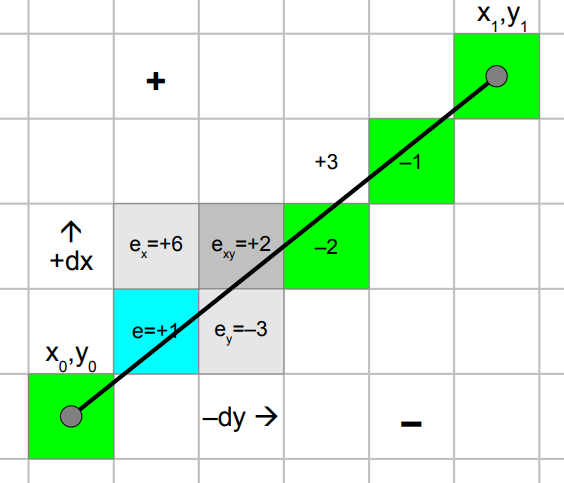
\includegraphics[width=0.5\linewidth]{img/Bresenhams}
%	\caption{Application of Bresenham's Algorithm to a straight line, %with visible errors. \cite{Zingl2012}}
%	\label{fig:collision_detection_bresenham}
%\end{figure}


\section{Implementation}
The collision detection logic is in effect every time a new point is added to the graph. The path planning algorithm samples a random point and calculates its nearest neighbour. After that, a function is called, which takes two points and checks for collision on a straight-line path between these two points.\newline
A problem that arises when using it this way is the not accounted for dimensions of the drone. For that, the function takes a third parameter defining the search radius. Using this method, paths can be generated suitable for the physical drone. However, this is accompanied by an increase in computational time, which stems from how this radius, $r$, is used. For every cell that is not the first and last cell, $2r$ neighbouring cells in a line opposite the line's direction get checked. For the first and last cell, the radius translates to the circle where cells get checked. In order to not overlap validation areas, on the first and last cell, only a semicircle is being covered. 

\begin{figure}[h]
	\centering
	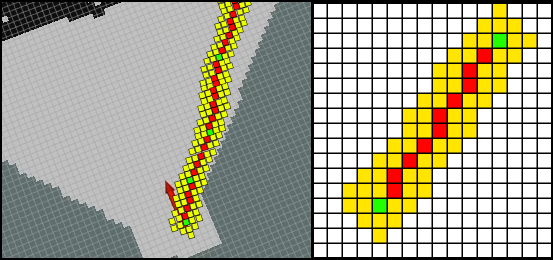
\includegraphics[width=0.8\linewidth]{img/CheckedPixels}
	\caption{Visualization of checked pixel in paths. Green being start/end points, red the lines calculated by the Bresenham's Algorithm and yellow the additionally checked cells with $r = 2$}
	\label{fig:collision_detection_checkedPixels}
\end{figure}

Therefore the to be checked cells can be calculated in dependency of the line length $l$ and radius $r$. $l$ thereby being the number of cells present in the line calculated by Bresenham's Algorithm. 
\[C=r^2+(l-2)*2r\]

\subsection{3 dimensional space}
Using this concept in a 3-dimensional environment only requires adding the new third dimension. Bresenham's Algorithm is easy to translate into the third¹2 dimension. The problem that arises is performance. When adding the radial search, it increases the total cells checked by \(C^2 - l\).  

\section{Experiment}

In order to be able to assess the practical impact of the collision detection performed by the autumn pathfinding algorithm, an experiment was conducted, which illustrates the computational time needed to guarantee no collisions from happening.

\subsection{Experimental Setup}

The experiment is split into two parts: the impact of collision detection on the computational time of two-dimensional and three-dimensional path-finding.
To get significant data, which can represent various scenarios in which the algorithm has to perform, a setup was selected to cover all aspects of the algorithm. The experiment works by planning a path through a static environment. This environment stays the same for all iterations of one algorithm and the two different variations of the algorithm. To get conclusive evidence concerning the collision detection, which is not polluted by the random nature of the algorithm, the sample size has been set to 100. \newline One sample refers thereby to a path planning with consistent parameters. The parameters are
\begin{itemize}
	\item the number of iterations of the RRT* algorithm($i$),
	\item the distance between the start and end node($d$), and
	\item the spacing of the nodes of the expanding tree($D$).
\end{itemize}
These three parameters stay constant throughout the entire duration of the experiment, the reason being that these three Parameters affect the parts of the path planning algorithm that aren't of concern in this experiment. The Parameter controlling the collision detection behaviour is the radius($r$).
For each radius, 100 paths are generated, and each execution of the algorithm is timed from the point of the function call till the return of the calculated path. 
The set of radii to be tested depends on the space in which paths are generated.
For each radius, the meantime of all 100 data points is calculated. This results in data representing how collision detection impacts the computational time of the autumn path-planning algorithm.

\subsection{Two-dimensional Algorithm}

For autumn\_pathplanning\_2d, radii starting from zero, resulting in disabling collision detection functionality, up to two 2000, with a step size of 100, have been tested. In figure \ref{plot:2dCollisionExp} the linear relationship between collision detection and the computational time can be observed. Furthermore, it can be derived from this plot that the two-dimensional path planning algorithm can handle high amounts of collision checks without making the path calculation unusable. On average, an additional 100 in radius results in a 90ms longer runtime. In this context, it should be pointed out that the radii chosen in this experiment are not in relation to radii used in practical application. For a 0.05 resolution of the occupancy grid used, radii in a range from 15 to 50 are practical. Nevertheless, this accentuated representation with a correlation coefficient of nearly one can also be applied to the practical values.   

\begin{figure}[h]
	\begin{center}
		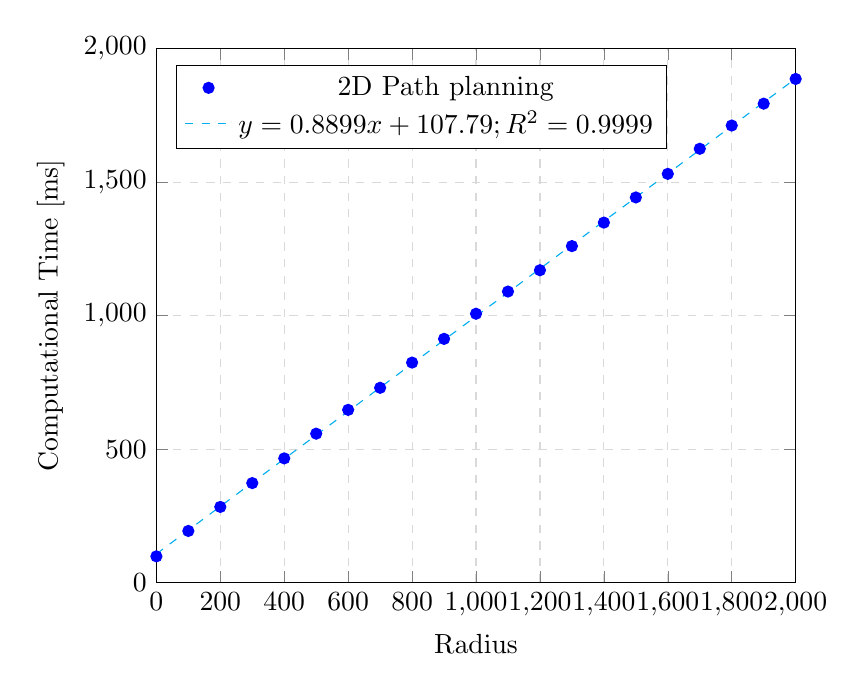
\begin{tikzpicture}
			\begin{axis}[
				width=0.8\linewidth, % Scale the plot to \linewidth
				grid=major, 
				grid style={dashed,gray!30},
				xlabel={Radius}, % Set the labels
				ylabel={Computational Time [ms]},
				legend pos=north west,
				xmin=0,
				xmax=2000,
				ymin=0,
				ymax=2000,
				]
				
				
				%2d test data
				\addplot[only marks, color=blue]
				table[row sep=crcr]{
					0 98.853165 \\
					100 193.98699\\
					200 283.95058\\
					300 373.10144\\
					400 465.5869\\
					500 558.11993\\
					600 647.20301\\
					700 729.78178\\
					800 824.24182\\
					900 912.9868\\
					1000 1007.04737\\
					1100 1090.12372\\
					1200 1169.9529\\
					1300 1260.2584\\
					1400 1348.2436\\
					1500 1442.4541\\
					1600 1530.6858\\
					1700 1624.6226\\
					1800 1711.6543\\
					1900 1793.4719\\
					2000 1885.9677\\
				}; 
				\addlegendentry{2D Path planning}
				
				%2d test regression
				\addplot[domain=0:2000, samples=100,no marks, color=cyan, style=dashed]
				{0.8899*x + 107.79};
				\addlegendentry{$y = 0.8899x + 107.79; R^2 =  0.9999$} 
			\end{axis}
		\end{tikzpicture}
		\caption{This plot illustrates the increase in computational time with increased collision detection, for the two-dimensional path-planning algorithm. Each point represents the average time needed to compute 100 paths, with equivalent parameters.}
		\label{plot:2dCollisionExp}
	\end{center}
\end{figure}

\subsection{Three-dimensional Algorithm}

The three-dimensional algorithm was tested with values ranging from $10$ to $320$, with an increment of $2^n * 10$. Figure \ref{plot:3dCollisionExp} illustrates the result of the experiment performed using the autumn\_pathplanning algorithm. The exponential relationship between the number of collision checks and computational time is apparent. With a block size of the point cloud of 0.01, the radii used in practice would range from 20 up to 150.

\begin{figure}[h]
	\begin{center}
		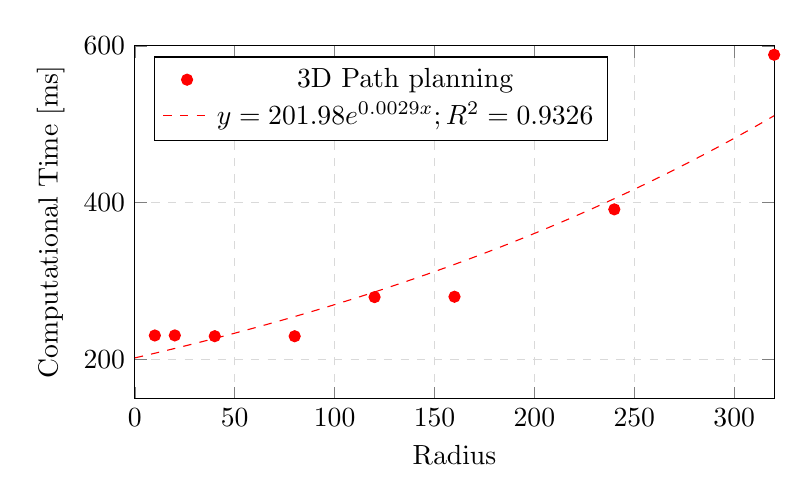
\begin{tikzpicture}
			\begin{axis}[
				height=0.5\linewidth,
				width=0.8\linewidth, % Scale the plot to \linewidth
				grid=major, 
				grid style={dashed,gray!30},
				xlabel={Radius}, % Set the labels
				ylabel={Computational Time [ms]},
				legend pos=north west,
				xmin=0,
				xmax=320,
				ymin=150,
				ymax=600,
				]
				
				
				%2d test data
				\addplot[only marks, color=red]
				table[row sep=crcr]{
					10 230.5572793  \\
					20 230.6465518  \\
					40 229.669491   \\
					80 229.5970721  \\
					120 279.5138153 \\
					160 279.9739437 \\
					240 391.4133536 \\
					320 588.5701149 \\
				}; 
				\addlegendentry{3D Path planning}
				
				%2d test regression
				\addplot[domain=0:320, samples=100,no marks, color=red, style=dashed]
				{201.98*e^(0.0029*x)};
				\addlegendentry{$y = 201.98e^{0.0029x}; R^2 =  0.9326$} 
			\end{axis}
		\end{tikzpicture}
		\caption{In this plot the correlation between increased collision detection and computational time, for the three-dimensional path-planning algorithm }
		\label{plot:3dCollisionExp}
	\end{center}
\end{figure}
